\section{Examples}

\subsection{Nomystery}

\subsubsection*{Explanation Domain}
The goal in nomystery is to deliver packages from an initial location 
to a goal location. There are two trucks with a separate fuel level.
The amount of packages a truck can transport is not limited. A truck can either load or 
unload a package or drive from one to another location. 

For this domain we consider the following properties, that will serve as the basis for addressing user questions:

\begin{itemize}
	\item uses $T_i$ $(L_x,L_y)$: Truck $T_i$ drives at least once from $L_x$ to
		$L_y$ or vice versa;
	\item doesn't use $T_i$ $(L_x,L_y)$: Truck $T_i$ does not drive from $L_x$ to
		$L_y$ or vice versa;
	\item same truck $P_x$ $P_y$: both packages are delivered by the same truck
		(the packages are either only loaded and an unloaded by truck $T_0$ or by $T_1$).
\end{itemize}

In this example we consider the problem shown in Figure, where all packages are in the initial location $L_0$ (labeled in red) and must be delivered in goal locations (labeled in green). 
Loading and unloading costs no fuel, while driving costs between 1 and 5 fuels units (as indicated by edge labels).\\
The amount of fuel available is 1.5 times higher than needed to deliver all packages; concretely, the initial fuel in trucks is $fuel(T_0) = 16$, $fuel(T_1) = 7$.


	\begin{center}
	\begin{tikzpicture}
		\node[draw, circle, label=above:{\textcolor{red}{$P_0, P_1,P_2$}}] (l0) at (0,0) {$L_0$};
		\node[draw, circle, label=right:{$T_1$}] (l1) at (4,-1) {$L_1$};
		\node[draw, circle] (l2) at (6,0) {$L_2$};
		\node[draw, circle, label=right:{\textcolor{darkgreen}{$P_1$}}] (l3) at (6,-3) {$L_3$};
		\node[draw, circle, label=below:{\textcolor{darkgreen}{$P_0$}}] (l4) at (2,-2) {$L_4$};
		\node[draw, circle, label=below:{$T_0$ \textcolor{darkgreen}{$P_2$}}] (l5) at (0,-3) {$L_5$};

		\draw[thick] (l0) to node[above] {5} (l2);
		\draw[thick] (l0) to node[above] {2} (l1);
		\draw[thick] (l0) to node[above] {3} (l4);
		\draw[thick] (l0) to node[left] {4} (l5);
		\draw[thick] (l2) to node[right] {1} (l3);
		\draw[thick] (l4) to node[above] {2} (l1);
		\draw[thick] (l4) to node[above] {5} (l3);
		\draw[thick] (l5) to node[below] {5} (l3);
		\draw[thick] (l4) to node[below] {4} (l5);
	\end{tikzpicture}
	\end{center}
	
Given the problem example, we then consider six instances of the properties above, and compute the corresponding set of MUGS.
	\smallskip
	\smallskip
	
	\begin{minipage}[t]{0.3\textwidth}
	Properties:
	\begin{enumerate}
		\item [\textbf{Pr1}] uses $T_0$ $(L_2,L_3)$
		\item [\textbf{Pr2}] same truck $P_1$ $P_2$
		\item [\textbf{Pr3}] uses $T_0$ $(L_4,L_3)$
		\item [\textbf{Pr4}] same truck $P_2$ $P_0$
		\item [\textbf{Pr5}] doesn't use $T_0$ $(L_0,L_5)$
		\item [\textbf{Pr6}] uses $T_1$ $(L_5,L_4)$
	\end{enumerate}
	\end{minipage}
	\begin{minipage}[t]{0.15\textwidth}
		MUGS:
		\begin{itemize}
			\item $\{4,5,6\}$
			\item $\{2,5,6\}$
			\item $\{3,4,5\}$
			\item $\{3,4,5\}$
			\item $\textbf{\{2,4,5\}}$
			\item $\{2,3,5\}$
			\item $\{1,3,4\}$
			\item $\{1,2,3\}$
		\end{itemize}
	\end{minipage}
	
The MUGS can then be used to generate explanations for plan inputs. In particular, each Pr\textit{i} corresponds to a possible action that a user would expect to see or not to see in the plan, and the MUGS are used to explain to the user that if they want one given action in the plan, then the user must necessarily change some other things in the plan, as guaranteed by the MUG. And this is an interesting kind of explanation/advice that also a non-planning person can understand. In more technical terms, the explanation informs the user about what properties they must relax in the plan in order to achieve what they want.

Let us assume we have the following plan that solves the problem of Figure  (in [] we put the fuel cost if greater than zero):

\begin{verbatim}
(drive T0 L5 L0) [4]
(load P0 T0 L0) 
(load P1 T0 L0) 
(load P2 T0 L0) 
(drive T0 L0 L4) [3]
(unload P0 T0 L4) 
(drive T0 L4 L5) [4]
(unload P2 T0 L5)
(drive T0 L5 L3) [5]
(unload P1 T0 L3)
\end{verbatim}

Given this plan, the user might ask \textit{''Why don't you avoid driving in the road $L_0-L_5$ as I know there is a lot of traffic there at the moment?"}. This question corresponds to forcing \textbf{Pr5} to be satisfied. At the same time, the plan already satisfies \textbf{Pr2} and \textbf{Pr4} given that only truck $T_0$ is used for all packages. However, one of the MUGS is \{2,4,5\}, and hence the answer to the user question would be: \textit{Because if you don't use that road, then you would not be able to deliver all packages using a single truck}.




\subsection{Blocksworld}

The cost bound is set to 11, 0.5 times the minimal cost to solve all goals.
You can pick up and put down a block from the table and stack and unstack two blocks.
Each of these actions costs 1.

\begin{center}
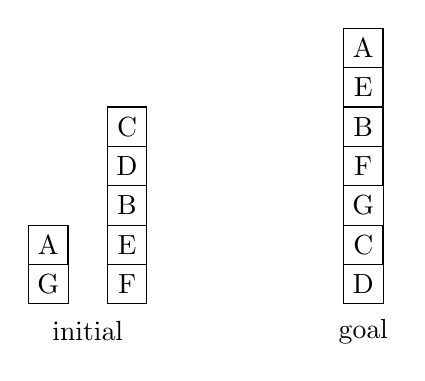
\begin{tikzpicture}
	\node[draw, minimum size=0.5cm] (G) at (0,0) {G};
	\node[draw, minimum size=0.5cm] (A) at (0,0.5) {A};

	\node[draw, minimum size=0.5cm] (F) at (1,0) {F};
	\node[draw, minimum size=0.5cm] (E) at (1,0.5) {E};
	\node[draw, minimum size=0.5cm] (B) at (1,1) {B};
	\node[draw, minimum size=0.5cm] (D) at (1,1.5) {D};
	\node[draw, minimum size=0.5cm] (C) at (1,2) {C};
	\node[] (i) at (0.5,-0.6) {initial};


	\node[draw, minimum size=0.5cm] (D) at (4,0) {D};
	\node[draw, minimum size=0.5cm] (C) at (4,0.5) {C};
	\node[draw, minimum size=0.5cm] (G) at (4,1) {G};
	\node[draw, minimum size=0.5cm] (F) at (4,1.5) {F};
	\node[draw, minimum size=0.5cm] (B) at (4,2) {B};
	\node[draw, minimum size=0.5cm] (E) at (4,2.5) {E};
	\node[draw, minimum size=0.5cm] (A) at (4,3) {A};
	\node[] (g) at (4,-0.6) {goal};
\end{tikzpicture}
\end{center}

MUGS:
\begin{itemize}
	\item $\{on(E,B), on(G,C)\}$
	\item $\{on(A,E), on(C,D), on(G,C)\}$
	\item $\{on(B,F), on(G,C)\}$
	\item $\{on(F,G)\}$
	\item $\{on(A,E), on(C,D), on(E,B)\}$
	\item $\{on(B,F), on(E,B)\}$
	\item $\{on(B,F), on(C,D)\}$
	\item $\{on(A,E), on(B,F)\}$
\end{itemize}


